\documentclass[12pt]{beamer}
\usetheme{default}
\usecolortheme{crane}
%\usetheme{Madrid}

\usepackage[utf8x]{inputenc}
\usepackage[T1]{fontenc}
\usepackage[slovak]{babel}
\usepackage{ucs}
\usepackage{amsmath}
\usepackage{graphicx}
\usepackage{array}
\usepackage{amsmath, amssymb}
\usepackage{hyperref, url}
%\usepackage[inline]{asymptote}

%\setbeamersize{text margin left=1pt,text margin right=1pt}
\setbeamertemplate{footline}[frame number]
\beamertemplatenavigationsymbolsempty

\let\o=\vee
\let\a=\wedge
\let\bigo=\bigvee
\let\biga=\bigwedge

\title{Databázové systémy}
\author{Ján Mazák}
\institute{FMFI UK Bratislava}
\date{}
%\date % (optional)
%{23. 9. 2019}

% database-related stuff
\DeclareMathOperator{\join}{\bowtie}
\DeclareMathOperator{\antijoin}{\rhd}

\DeclareMathOperator{\COUNT}{\textrm{COUNT}}
\DeclareMathOperator{\SUM}{\textrm{SUM}}
\DeclareMathOperator{\MAX}{\textrm{MAX}}


\DeclareMathOperator{\osoba}{osoba}
\DeclareMathOperator{\firma}{firma}
\DeclareMathOperator{\vlastni}{vlastni}
\DeclareMathOperator{\ponuka}{ponuka}
\DeclareMathOperator{\chce}{chce}
\DeclareMathOperator{\lubi}{lubi}
\DeclareMathOperator{\capuje}{capuje}
\DeclareMathOperator{\navstivil}{navstivil}
\DeclareMathOperator{\vypil}{vypil}
\DeclareMathOperator{\answer}{answer}


\begin{document}

\frame{\titlepage}

\begin{frame}{Čo je databáza?}
\begin{itemize}
\item kolekcia údajov
\item so štruktúrou
\end{itemize}
\vskip 1cm
\pause

DBMS (database management system), voľne tiež databáza
\begin{itemize}
\item obsahuje veci spoločné pre jednotlivé databázy
\item pracuje nad dátami abstraktne, používateľ (tvorca konkrétnej databázy) definuje všetky vzťahy medzi dátami (napr. konzistentnosť)
\end{itemize}
\end{frame}

\begin{frame}{Požiadavky na DBMS}
\begin{itemize}
\item trvalé uchovanie (persistency)
\item bezpečnosť (na úrovni hw, sw, používateľov)
\item paralelizmus (veľa používateľov zároveň)
\item pohodlnosť (vysokoúrovňové deklaratívne jazyky)
\item efektívnosť (tisíce dotazov za sekundu)
\end{itemize}
\bigskip
\pause
Aplikácie zapisujúce extrémne množstvo dát neraz nevyužívajú DBMS, lebo by ich to spomalilo.
\end{frame}

\begin{frame}{Čo všetko súvisí s DBMS?}
\begin{itemize}
\item fyzické umiestnenie dát (HDD vs. SSD, súborový systém)
\item sieťové pripojenia (klienti, distribuovanosť databázy)
\item paralelizmus (veľa používateľov robiacich operácie nad tými istými dátami)
\item optimalizácia dotazov (algoritmická zložitosť)
\end{itemize}
\end{frame}

\begin{frame}{Multitier architecture}
\begin{itemize}
\item 1-tier: používateľ/aplikačný program pracuje priamo s db (napr. androidová aplikácia s SQLite)
\item 2-tier: používateľ k db pristupuje cez sieť, ale priamo
\pause
\item 3-tier: bežné webové aplikácie: frontend a backend, používateľ nekomunikuje priamo s db a všetka komunikácia ide cez API backendu\\
	(možno napr. filtrovať dáta podľa prihláseného užívateľa nad rámec databázového dotazu)
\end{itemize}
\end{frame}


\begin{frame}{Dátový model}
\begin{itemize}
\item relačný (tabuľky)
\item entitno-relačný
\item objektový
\item hierarchický (strom)
\item dokumentový (XML, json)
\item graf
\item key-value store
\end{itemize}
\bigskip
SQL --- relačný model\\
NoSQL --- key-value store, graph, document...
\end{frame}

\begin{frame}{Relačný dátový model}
Dáta v tabuľkách; stĺpce sú atribúty, riadky záznamy.

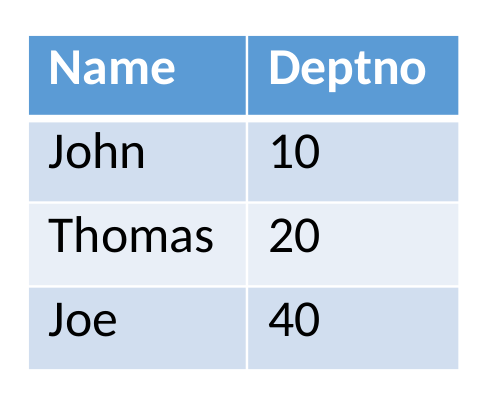
\includegraphics[scale=.25]{rel1.png}
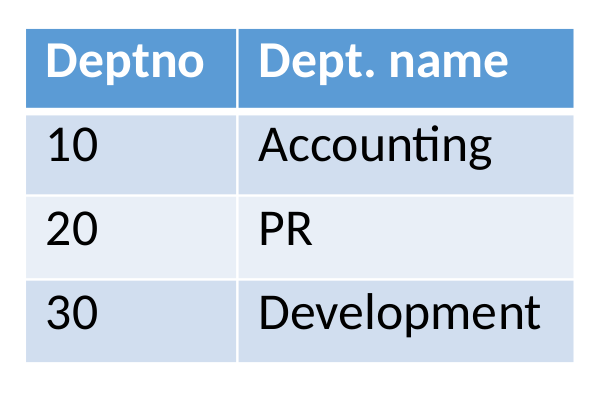
\includegraphics[scale=.25]{rel2.png}

Záznamy z rôznych tabuliek sa prepájajú operáciou JOIN.
\end{frame}

\begin{frame}{Databázové jazyky}
\begin{itemize}
\item Data Query Language (DQL) --- dotazy
\item Data Definition Language (DDL) --- definovanie štruktúry db
\item Data Manipulation Language (DML) --- vkladanie, mazanie a úprava dát
\end{itemize}
\vskip 1 cm
\pause
Prístup k dátam z programovacích jazykov:
\begin{itemize}
\item priamo (cez DML)
\item s jednoduchou nadstavbou (prepared statement atď.)
\item ORM (object-relational mapper) --- pracuje sa s objektmi, DML sa automaticky generuje v pozadí 
\end{itemize}
\end{frame}

\begin{frame}{Dotazovacie jazyky}
\begin{itemize}
\item chceme, aby aplikácie boli nezávislé od reprezentácie dát
\item optimalizácia na úrovni DBMS, nie u klienta
\pause
\item deklaračné jazyky (len čo chceme, nie ako to vypočítať): relačný kalkul (prvorádové matematické formuly), SQL, Datalog
\pause
\item interné db jazyky (procedurálne zachytávajú postup výpočtu): relačná algebra, fyzické operátory
\end{itemize}
\end{frame}

\begin{frame}{Nevhodnosť prirodzeného jazyka}
Ľudia neraz veci kvantifikujú nesprávne alebo neúplne (zvlášť pozor na ľudí pôsobiacich v inom odvetví, kde nepoznáte konvencie).
Ako interpretovať tvrdenie \uv{chlieb predávajú v potravinách}?
\pause
\begin{itemize}
\item každý chlieb predávajú len v potravinách a nikde inde
\item existuje druh chleba, ktorý predávajú len v miestnej predajni potravín
\item existuje druh chleba, ktorý predávajú v každých potravinách
\item existujú potraviny, ktoré predávajú aspoň jeden chlieb
\item každé potraviny predávajú aspoň jeden chlieb
\item \dots
\end{itemize}
\end{frame}

\begin{frame}{Ukážka relač. kalkulu, datalogu a relačnej algebry}
Alkoholy, ktoré ľúbi každý pijan (ktorý niečo ľúbi), čapujú ich všade (kde niečo čapujú) a niekto ich už pil.

{\scriptsize
\begin{align*}
\Big\{A\mid (\exists I\,\exists M\vypil(I, A, M))&\land \lnot \Big[\exists P (\exists A_2\lubi(P, A_2))\land\lnot\lubi(P, A))\Big)\Big]\\
&\land \lnot\Big[\exists K \Big((\exists A_2 \capuje(K, A_2))\land \lnot\capuje(K, A)\Big)\Big]\Big\}
\end{align*}
}
{\scriptsize
\begin{align*}
\operatorname{nelubenyNiekym}(A) &\leftarrow \vypil(\_, A, \_), \lubi(P, \_), \lnot\lubi(P, A).\\
\operatorname{necapovanyNiekde}(A) &\leftarrow \vypil(\_, A, \_), \capuje(K, \_), \lnot\capuje(K, A).\\
\answer(A) &\leftarrow \vypil(\_, A, \_), \lnot\operatorname{nelubenyNiekym}(A), \lnot\operatorname{necapovanyNiekde}(A).\\
\end{align*}
}
\vskip -2mm
\vskip -2mm
{\scriptsize
\begin{align*}
\operatorname{nelubenyNiekym} & = (\pi_A(\vypil)\times \pi_P(\lubi))\antijoin \lubi\\
\operatorname{necapovanyNiekde} & = (\pi_A(\vypil)\times \pi_K(\capuje))\antijoin \capuje\\
\answer & = ((\pi_A(\vypil) \antijoin \operatorname{nelubenyNiekym})\antijoin \operatorname{necapovanyNiekde}\\
\end{align*}
}
\end{frame}

\begin{frame}[fragile]
\frametitle{Ukážka SQL}
Alkoholy, ktoré ľúbi každý pijan (ktorý niečo ľúbi), čapujú ich všade (kde niečo čapujú) a niekto ich už pil.

{\scriptsize
\begin{verbatim}
    SELECT DISTINCT v.A
    FROM vypil v
    WHERE NOT EXISTS (SELECT 1 FROM lubi l
                      WHERE NOT EXISTS (SELECT 1 FROM lubi l2
                                        WHERE l2.P = l.P AND l2.A = v.A))
        AND NOT EXISTS (SELECT 1 FROM capuje c
                        WHERE NOT EXISTS (SELECT 1 FROM capuje c2
                                        WHERE c2.K = c.K AND c2.A = v.A))
\end{verbatim}
}
\end{frame}

\begin{frame}
\frametitle{História}
\begin{itemize}
\item 1970: relačný model
\item 1986: prvý štandard SQL
\item od cca 2010: NoSQL, Spark...
\pause
\item reálne systémy nedržia tempo s teóriou ani SQL štandardmi, napr. rekurzia je v najväčších DBMS implementovaná ani 10 rokov, kým štandard je z 1999
\item a naopak k NoSQL systémom chýba univerzálna formálna teória (sú rôznorodé)
\end{itemize}
\end{frame}

\begin{frame}
\frametitle{NoSQL databázy}
\begin{theorem}[CAP theorem, proved in 2002]
Neexistuje systém, ktorý má zároveň tieto 3 vlastnosti:
\begin{itemize}
\item consistency
\item availability
\item partition tolerance
\end{itemize}
\end{theorem}
\begin{itemize}
\item[CP:] MongoDB
\item[AP:] Cassandra
\item[CA:] partitions cannot be avoided, but PostgreSQL (somewhat)
\end{itemize}
{\scriptsize Viac: \url{https://www.ibm.com/topics/cap-theorem}}
\end{frame}


\begin{frame}{Databases used by professionals (2022)}
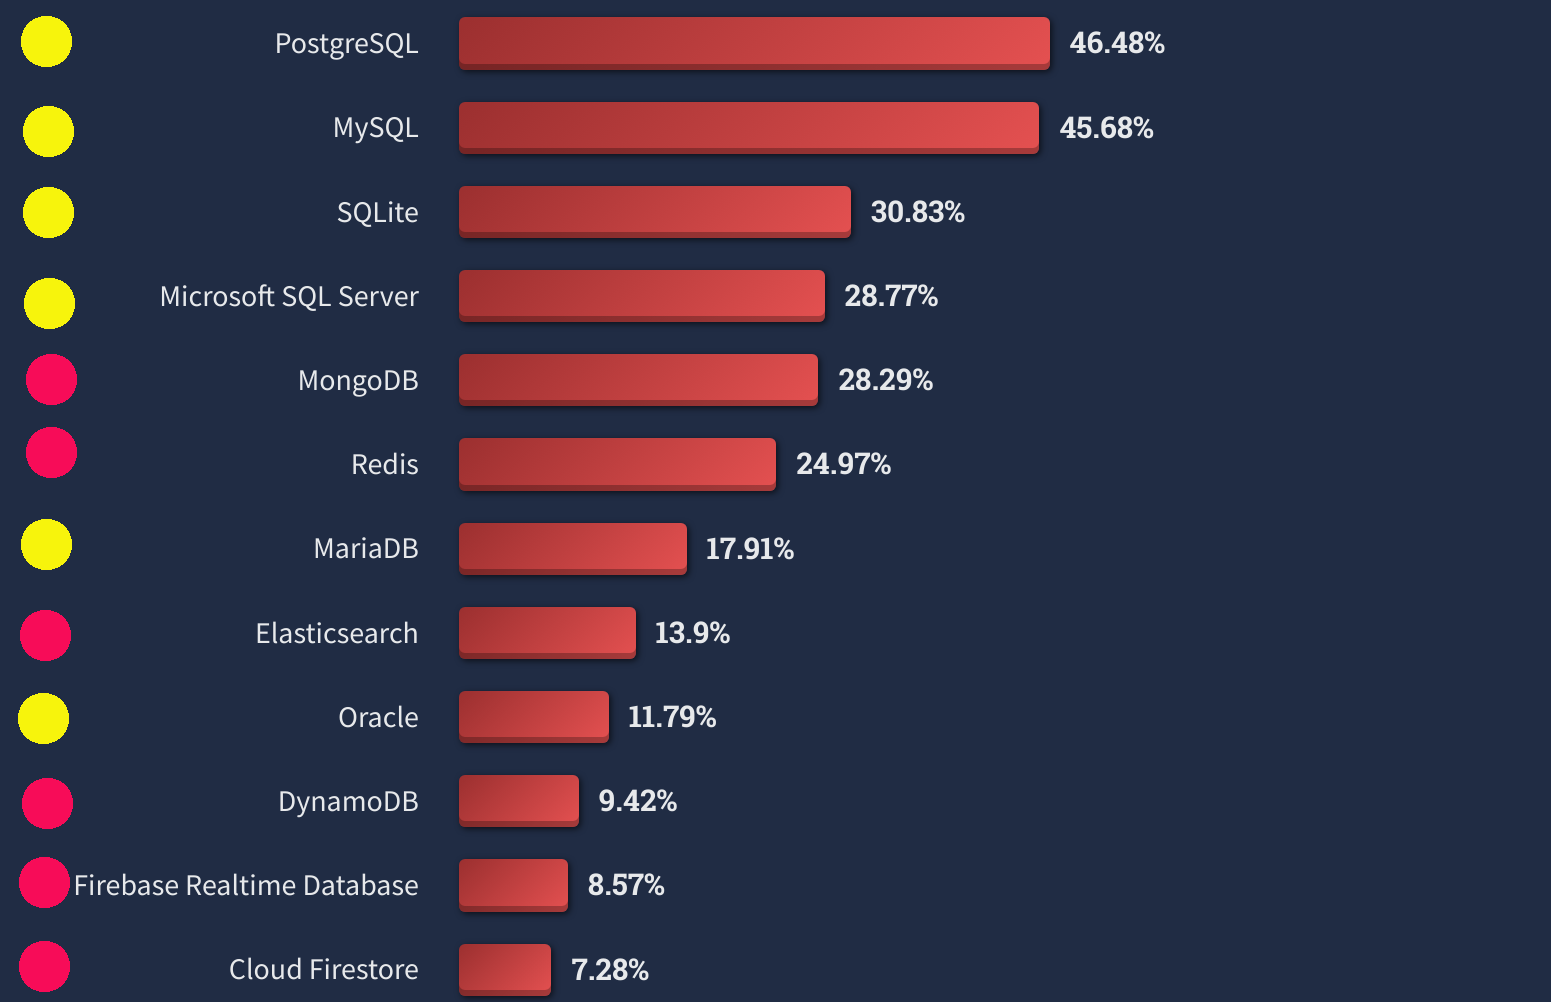
\includegraphics[scale=.15]{commondb_modified.png}\\
{\tiny \url{https://survey.stackoverflow.co/2022/}}\\[3mm]
{\small yellow --- relational databases (SQL)}\\
{\small others --- not relational, NoSQL}
\end{frame}

\begin{frame}{DBMS na tomto predmete}
PostgreSQL
\begin{itemize}
\item výborný súlad s SQL štandardom
\item zrozumiteľná a podrobná dokumentácia
\item dobrý výkon, škálovateľnosť, široké využitie v praxi
\end{itemize}
\bigskip

SQLite
\begin{itemize}
\item celá databáza v jedinom súbore
\item ľahko prenosná, zálohovateľná a administrovateľná
\item nenáročná na pamäť i procesor
\item chýbajú mnohé veci bežné v iných DBMS
\end{itemize}
\end{frame}

\begin{frame}{Tento predmet}
\begin{itemize}
\item zameraný najmä na praktické aspekty práce s relačnými DBMS
\item dotazy
\item navrhovanie databázových schém v relačnom modeli
\item transakcie
\item efektivita (význam indexov, vkladanie veľkých objemov dát)
\pause
\item ale aj prehľad o teoretických aspektoch (vyjadrovacia sila dotazovacích jazykov, zložitosť vybraných algoritmov)
\end{itemize}
\end{frame}

\begin{frame}
\frametitle{Hodnotenie}
\begin{itemize}
\item účasť na prednáškach ani cvičeniach nie je povinná
\item prednášky zväčša zahŕňajú aj \uv{teoretické precvičenie}
\item cvičenia sú praktické, dajú sa robiť samostatne vo zvolenom čase; z každého treba spraviť aspoň časť\\ (10 x 2 b, treba min. 15)
\item tri domáce úlohy (3 x 20 b)
\item za semester 80 bodov
\item ústna skúška za 20 bodov, treba min. 10
\end{itemize}
\end{frame}


\begin{frame}{Literatúra}
\begin{itemize}
\item DBMS:\\
{\scriptsize\url{http://www.noucamp.org/cp2/dbt/DBIntroduction.pdf}}
{\scriptsize\url{https://www.db-book.com/slides-dir/PDF-dir/ch1.pdf}}
{\scriptsize\url{http://infolab.stanford.edu/~ullman/fcdb/ch1.pdf}}
{\scriptsize\url{https://www.ibm.com/topics/cap-theorem}}

\item SQL (zatiaľ len SELECT, WHERE, EXISTS):\\
{\scriptsize\url{https://www.w3schools.com/sql/sql_intro.asp}}\\
{\scriptsize\url{https://sqlbolt.com/lesson/select_queries_introduction}}\\
{\scriptsize\url{https://www.learnsqlonline.org/}}\\
\end{itemize}
\end{frame}


\begin{frame}{Úlohy: relačný kalkul}
Databáza: \emph{osoba}(A), \emph{pozna}(Kto, Koho)
\begin{itemize}
    \item osoby, ktoré poznajú sysľa
    \item osoby, ktoré nepoznajú nikoho (žiadne iné osoby)
    \item osoby, ktoré majú aspoň dvoch známych (osoby)
    \item osoby, ktoré pozná presne jedna osoba
    \item osoby, ktoré poznajú iba Jožka
    \item osoby, ktoré poznajú všetkých známych svojich známych
    \item osoby, ktoré majú všetky vzťahy symetrické
\end{itemize}
\end{frame}


\end{document}


